\ejercicio
\textit{Voy a estar usando las siguientes propiedades en $G_n$: }\\
Si $w \en G_n \entonces
	\llave{l}{
		w^n = 1 \entonces w^k = w^{r_n(k)}\\
		\conj w^k = w^{r_n(-k)} \\
		\sumatoria{k=0}{n-1}w^k = 0\\
		m \divideA n \entonces G_m \subseteq G_n,\text{ lo uso para saber con cuales raíces hay que tener cuidado}\\
		\text{Si } w \en G_p \text{ con $p$ primo } \entonces w \text{ es primitiva}
		w^k \text{es primitiva} \sisolosi k \cop n
	}$\\

\begin{enumerate}[label=\roman*)]
	\item Calcular $w + \conj w + (w + w^2)^2 - w^{38}(1 - w^2)$ para cada $w \en G_7$.

	      \separadorCorto
	      Raíces de $G_7$ de interés: 7 es primo e impar $\entonces w = 1$ se hace a parte.\\
	      \textit{Si} $w = 1$: \\
	      $w + \conj w + (w + w^2)^2 - w^{38}(1 - w^2) = 6$\\

	      \textit{Si} $w \distinto 1$: \\
	      $w + \ub{\conj w}{w^6} + (w + w^2)^2 - w^{38}(1 - w^2) =
		      w + w^6 + w^2 + 2w^3 + w^4 - \ub{(w^7)^5}{=1} w^3(1 - w^2) =\\
		      =  \magenta{-1} + \ub{\magenta{1} + w + w^2 + w^3 + w^4 + w^5 + w^6}{=0} = -1 \Tilde$

	\item Calcular $w^{73} + \conj w \cdot w^9 + 8$ para cada $w\en G_3$.

	      \separadorCorto
	      Raíces de $G_3$ de interés: 3 es primo e impar $\entonces w = 1$ se hace a parte.\\
	      \textit{Si} $w = 1$: \\
	      $w^{73} + \conj w \cdot w^9 + 8 = 10 $\\

	      \textit{Si} $w \distinto 1$: \\
	      $\ub{w^{73}}{w} + \ub{\conj w \cdot w^9 }{w^2 \cdot 1}+ 8 =
		      \magenta{-1} + \ub{\magenta{1} + w + w^2}{= 0} + 8 = 7 $

	\item Calcular $1 + w^2 + w^{-2} + w^4 + w^{-4}$ para cada $w\en G_{10}$.

	      \separadorCorto
	      % \red{Me falta harto golpe de horno para entender lo que pasa acá}\\
	      % \red{¿Cómo tengo que interpretar la info de $G_5 \subseteq G_{10}$ está proveyendo?}\\
	      Raíces de $G_{10}$ de interés: $2 \divideA 10 \y 5 \divideA 10$. $10$ es par $\entonces w = \pm1$ y
	      raíces de $G_2$ y de $G_5$ se hacen a parte.\\

	      \begin{minipage}{0.6\textwidth}
		      \begin{itemize}
			      \item \textit{Si} $w = \pm1$: \\
			            $1 + w^2 + w^{-2} + w^4 + w^{-4} = 5$ \Tilde\\

                      \item \textit{Si} $w \en G_{10} \text{ y } w \distinto \pm 1$: \\
			            $ 1 + w^2 + w^{-2} + w^4 + w^{-4} = 1 + w^2 + w^8 + w^4 + w^6 =\\
                        = \sumatoria{k=0}{4} (w^2)^k = \frac{(w^2)^5 - 1}{w^2 - 1} = 
                        \frac{\ob{\scriptstyle w^{10}}{=1} - 1}{w^2 - 1} = 0$
		      \end{itemize}



	      \end{minipage}
	      \begin{minipage}{0.35\textwidth}
		      \centering
		      $G_5 \subseteq G_{10}$\\
		      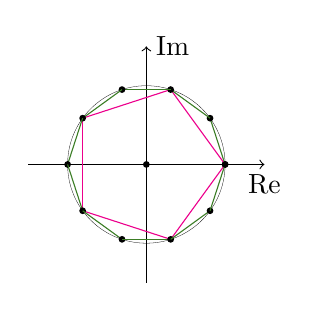
\begin{tikzpicture}[baseline=0]
			      \draw[->] (-1.5,0) -- (1.5,0) node[below] {Re};
			      \draw[->] (0,-1.5) -- (0,1.5) node[right] {Im};
			      \draw[ultra thin] (0,0) circle (1);
			      \filldraw[thin] (0,0) circle (1pt); % Added the origin
			      \foreach \x in {0,...,10} {
					      \filldraw (\x*360/10:1) circle (1pt);
					      \ifnum\x<10
						      \draw[OliveGreen] (\x*360/10:1) -- ({(\x+1)*360/10}:1);
					      \fi
					      \ifnum\x<5
						      \draw[magenta] (\x*360/5:1) -- ({(\x+1)*360/5}:1);
					      \fi
				      }
		      \end{tikzpicture}

		      $"G_5" \subseteq G_{10}$\\
		      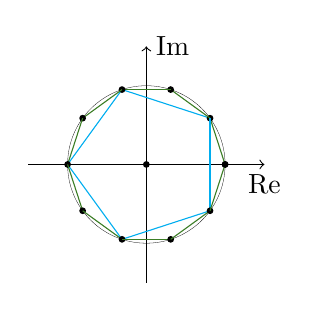
\begin{tikzpicture}[baseline=0]
			      \draw[->] (-1.5,0) -- (1.5,0) node[below] {Re};
			      \draw[->] (0,-1.5) -- (0,1.5) node[right] {Im};
			      \draw[ultra thin] (0,0) circle (1);
			      \filldraw[thin] (0,0) circle (1pt); % Added the origin

			      \foreach \x in {0,...,10} {
					      \filldraw (\x*360/10:1) circle (1pt);
					      \ifnum\x<10
						      \draw[OliveGreen] (\x*360/10:1) -- ({(\x+1)*360/10}:1);
					      \fi
					      \ifnum\x<5
						      \draw[cyan] ({\x*360/5+360/10}:1) -- ({(\x+1)*360/5+360/10}:1);
					      \fi
				      }
		      \end{tikzpicture}\\
	      \end{minipage}

	\item Calcular $w^{14} + w^{-8} + \conj w^4 + \conj{w^{-3}}$ para cada $w \en G_5$

	      \separadorCorto
	      \textit{Si} $w = 1$: \\
	      $w^{14} + w^{-8} + \conj w^4 + \conj{w^{-3}} = 4$

	      \textit{Si} $w \distinto 1$: \\
	      $w^{14} + w^{-8} + \conj w^4 + \conj{w^{-3}} =
		      w^4 + w^2 + w + w^3 =
		      \magenta{-1} + \ub{\magenta{1} + w + w^2 + w^3 + w^4}{= 0} = -1 $


\end{enumerate}
